\documentclass[aspectratio=169,28pt]{beamer}

\usepackage[utf8]{inputenc}
\usepackage[czech]{babel}
\usepackage{graphicx}
\usetheme{Madrid}
\usecolortheme{whale}
\usepackage[inline]{enumitem}

\setbeamercolor{normal text}{fg=black,bg=white}

\beamertemplatenavigationsymbolsempty
\makeatletter
\defbeamertemplate*{footline}{Dan P theme}
{
  \leavevmode%
  \hbox{%
  \begin{beamercolorbox}[wd=.25\paperwidth,ht=2.25ex,dp=1ex,center]{author in head/foot}%
    \usebeamerfont{author in head/foot}\insertshortauthor\expandafter\beamer@ifempty\expandafter{\beamer@shortinstitute}{}{~~(\insertshortinstitute)}
  \end{beamercolorbox}%
  \begin{beamercolorbox}[wd=.65\paperwidth,ht=2.25ex,dp=1ex,center]{title in head/foot}%
    \usebeamerfont{title in head/foot}\insertshorttitle
  \end{beamercolorbox}%
  \begin{beamercolorbox}[wd=.1\paperwidth,ht=2.25ex,dp=1ex,right]{date in head/foot}%
    \usebeamerfont{date in head/foot}\insertshortdate{}\hspace*{2em}
\insertframenumber{} / \inserttotalframenumber\hspace*{2ex} 
  \end{beamercolorbox}}%
  \vskip0pt%
}
\makeatother


\title{Semestrální práce z MI-EDW}
\subtitle{Educational Process Mining (EPM)}
\author{Ladislav Martínek a Richard Werner}
\date {}

\begin{document}

\section{Úvod}
\begin{frame}
\titlepage
\end{frame}

\section{Cíle}
\begin{frame}{Cíle}
\begin{itemize}
        \item[•] Analýza dat
		\item[•] Návrh a implementace datového skladu
		\item[•] Vytvoření dashboardu pro prezentaci dat
		\item[•] Zodpovězení business otázek
		\end{itemize}
\begin{columns}[c]
    \column{5cm}
    \column{10cm}
 \end{columns}   
      
\end{frame}

\section{Návrh a implementace}
\begin{frame}{Návrh a implementace}
		\begin{columns}[c]
    \column{8cm}
    \begin{itemize}
        \item[•] Analýza dat
		\item[•] Návrh a implementace datového skladu
		\item[•] Vytvoření dashboardu pro prezentaci dat
		\item[•] Zodpovězení business otázek
		\end{itemize}
    \column{7cm}
    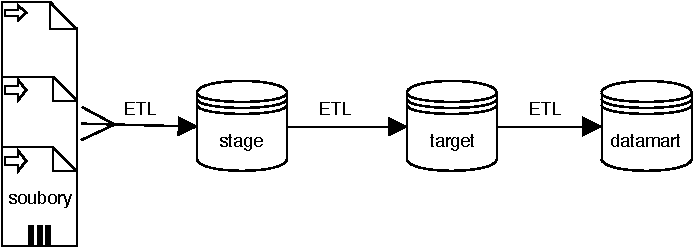
\includegraphics[scale=0.58]{img/DW}
 \end{columns}   
\end{frame}


\section{dashboard}
\begin{frame}{Dashboard}

\begin{columns}[c]
    \column{5cm}
    
    \column{10cm}
 \end{columns}   
		
\end{frame}

\section{Shrnutí}
\begin{frame}{Shrnutí}
		\begin{itemize}
		\item[•] ...
		\item[•] ...
		\item[•] ...
		\end{itemize}
\end{frame}


%\begin{frame}
%		\Huge\center{Děkuji za pozornost!}
%		\vskip 15pt
%		{\color{blue}\rule[2pt]{0.8\textwidth}{2pt}}
%		\color{black}\vskip 15pt
%		\LARGE\center{Dotazy?}
%\end{frame}


\end{document}

